\documentclass{exam}
\usepackage{graphicx}
\usepackage[utf8]{inputenc}
\usepackage[main=english, vietnamese]{babel}
\usepackage{amsmath}
\usepackage{hyperref}
\usepackage{amsthm}
\usepackage{tcolorbox}
\usepackage{amsfonts}
\usepackage{amssymb}
\usepackage{mathrsfs}
\usepackage{centernot}
\usepackage{multicol}
\usepackage{cases}
\usepackage{physics}
\usepackage[shortlabels]{enumitem}
\usepackage{tasks}
\usepackage{listings}

\definecolor{borderblue}{HTML}{33c2ff}
\definecolor{codegreen}{rgb}{0,0.6,0}
\definecolor{codegray}{rgb}{0.5,0.5,0.5}
\definecolor{codepurple}{rgb}{0.58,0,0.82}
\definecolor{backcolour}{rgb}{0.95,0.95,0.92}

\lstdefinestyle{mystyle}{
    backgroundcolor=\color{backcolour},   
    commentstyle=\color{codegreen},
    keywordstyle=\color{magenta},
    numberstyle=\tiny\color{codegray},
    stringstyle=\color{codepurple},
    basicstyle=\ttfamily\footnotesize,
    breakatwhitespace=false,         
    breaklines=true,                 
    captionpos=b,                    
    keepspaces=true,                 
    numbers=left,                    
    numbersep=5pt,                  
    showspaces=false,                
    showstringspaces=false,
    showtabs=false,
    tabsize=2
}

\lstset{style=mystyle}

\newcommand{\paren}[1]{\left(#1\right)}
\newcommand{\curly}[1]{\left\{#1\right\}}
\newcommand{\lxor}{\oplus}

\allowdisplaybreaks

\makeatletter
\renewcommand*\env@matrix[1][*\c@MaxMatrixCols c]{%
  \hskip -\arraycolsep
  \let\@ifnextchar\new@ifnextchar
  \array{#1}}
\makeatother

\makeatletter
\long\def\paragraph{%
  \@startsection{paragraph}{4}%
  {\z@}{2ex \@plus 1ex \@minus .2ex}{-1em}%
  {\normalfont\normalsize\bfseries}%
}
\makeatother

\makeatletter
\def\@xequals@fill{\arrowfill@\Relbar\Relbar\Relbar}
\newcommand*\xequals[2][]{\DOTSB\ext@arrow0055\@xequals@fill{#1}{#2}}
\makeatother

\DeclareMathOperator{\lcm}{lcm}
\DeclareMathOperator{\spn}{span}
\DeclareMathOperator{\im}{im}
\DeclareMathOperator{\nullity}{nullity}

\newbox\mizukibox
\setbox\mizukibox\hbox{
\raisebox{-2.5pt}{
\includegraphics[height=2.5ex]{mizuki.png}}}
\def\mizuki{\copy\mizukibox}

\newbox\skullbox
\setbox\skullbox\hbox{
\raisebox{-2.5pt}{
\includegraphics[height=2.5ex]{skull.png}}}
\def\bendingskull{\copy\skullbox}

\makeatletter
\renewcommand*\env@matrix[1][*\c@MaxMatrixCols c]{%
  \hskip -\arraycolsep
  \let\@ifnextchar\new@ifnextchar
  \array{#1}}
\makeatother

\NewTColorBox{problem}{m}{
  standard jigsaw,
  sharp corners,
  boxrule=0.4pt,
  coltitle=black,
  colframe=black,
  opacityback=0,
  opacitybacktitle=0,
  fonttitle=\normalfont\bfseries\upshape,
  fontupper=\normalfont,
  title={Problem #1},
  after title={.},
  attach title to upper={\ },
}

\renewcommand\qedsymbol{$\mizuki$}

\title{STAT451 - Homework 1}
\author{\foreignlanguage{vietnamese}{Trần Tôn Minh Kỳ}}
\date{\today}

\begin{document}

\maketitle
\begin{problem}{71}
	Here is a description from Minitab of the strength data  given in Exercise 13.
	\begin{lstlisting}
		Variable	N		Mean		Median		TrMean		StDev		SE Mean
		strength	153	135.39	135.40		135.41		4.59		0.37
		
		Variable	Minimum		Maximum		Q1				Q3
		strength	122.20		147.70		132.95		138.25
	\end{lstlisting}
	\begin{tasks}[label=\textbf{\alph*.}]
		\task Comment on any interesting features (the quartiles and fourths are virtually identical here).
		\task Construct a boxplot of the data based on the quartiles, and comment on what you see.
	\end{tasks}
\end{problem}

\paragraph{\textbf{a.}} Because the mean is lower than the median, we can see that the distribution of the data is roughly negatively skewed. However, they are also close to each other, which suggests a rough symmetry. Judging the interquartile range, the minimum and maximum are most likely outliers which affects the mean and standard deviation.

\paragraph{\textbf{b.}} The box plot is given below

\begin{minipage}{0.35\textwidth}
	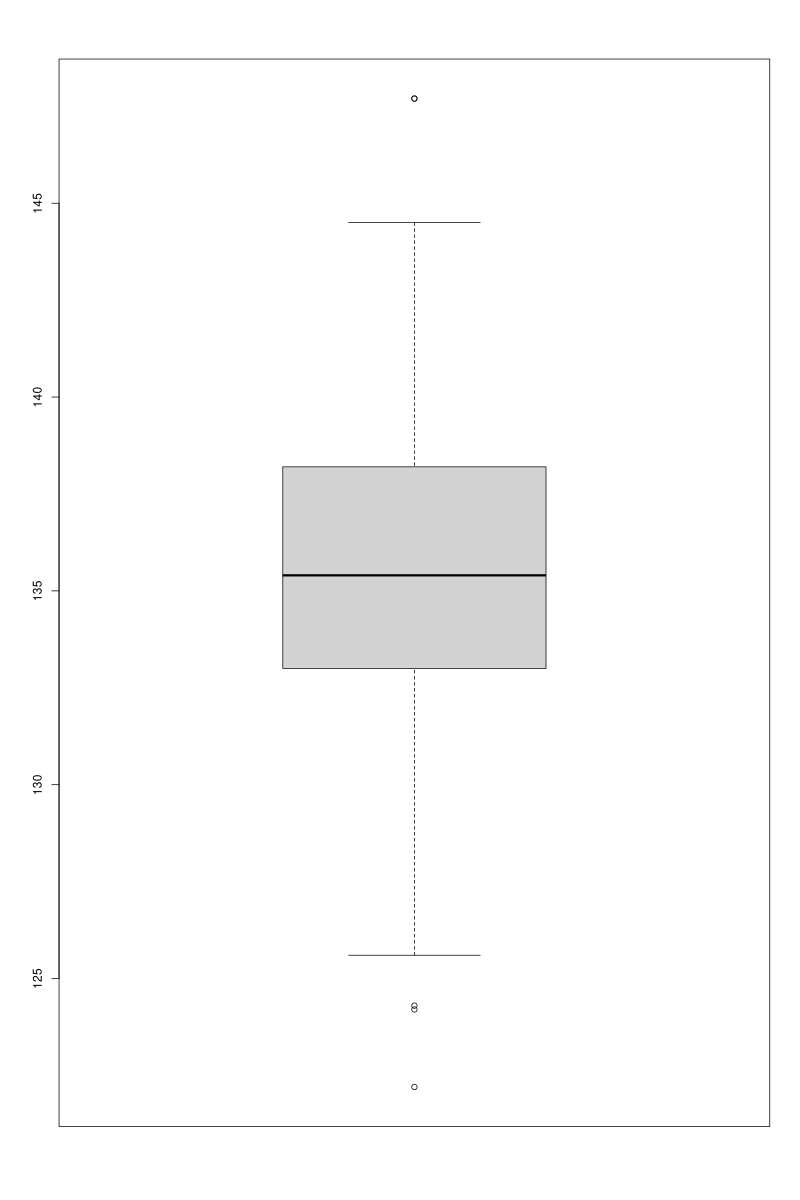
\includegraphics[scale=0.2]{img/71b.png}
\end{minipage}
\begin{minipage}{0.58\textwidth}
	Looking at the boxplot, we can see the box itself is approximately located at the middle of both whisker ends, with a very slight skew towards the upper whisker. Additionally, the box itself has a fair width, indicating a fair variability in the dataset. There are visible outliers at both whisker ends.
\end{minipage}

\begin{problem}{72}
	Anxiety disorders and symptoms can often be effectively treated with benzodiazepine medications. It is known that animals exposed to stress exhibit a decrease in benzodiazepine receptor binding in the frontal cortex. The article \textbf{``Decreased Benzodiazepine Receptor Binding in Prefrontal Cortex in Combat-Related Posttraumatic Stress Disorder'' (\textit{Amer. J. of Psychiatry, 2000: 1120--1126})} described the first study of benzodiazepine receptor binding in individuals suffering from PTSD. The accompanying data on a receptor binding measure (adjusted distribution volume) was read from a graph in the article.
	\begin{description}[style=multiline, leftmargin=1.5cm, font=\normalfont\textit]
		\item[PTSD:] 10, 20, 25, 28, 31, 35, 37, 38, 38, 39, 39, 42, 46
		\item[Healthy:] 23, 39, 40, 41, 43, 47, 51, 58, 63, 66, 67, 69, 72
	\end{description}
	Use various methods from this chapter to describe and summarize the data.
\end{problem}

Using box plots, we obtain the following:

\begin{minipage}{0.35\textwidth}
	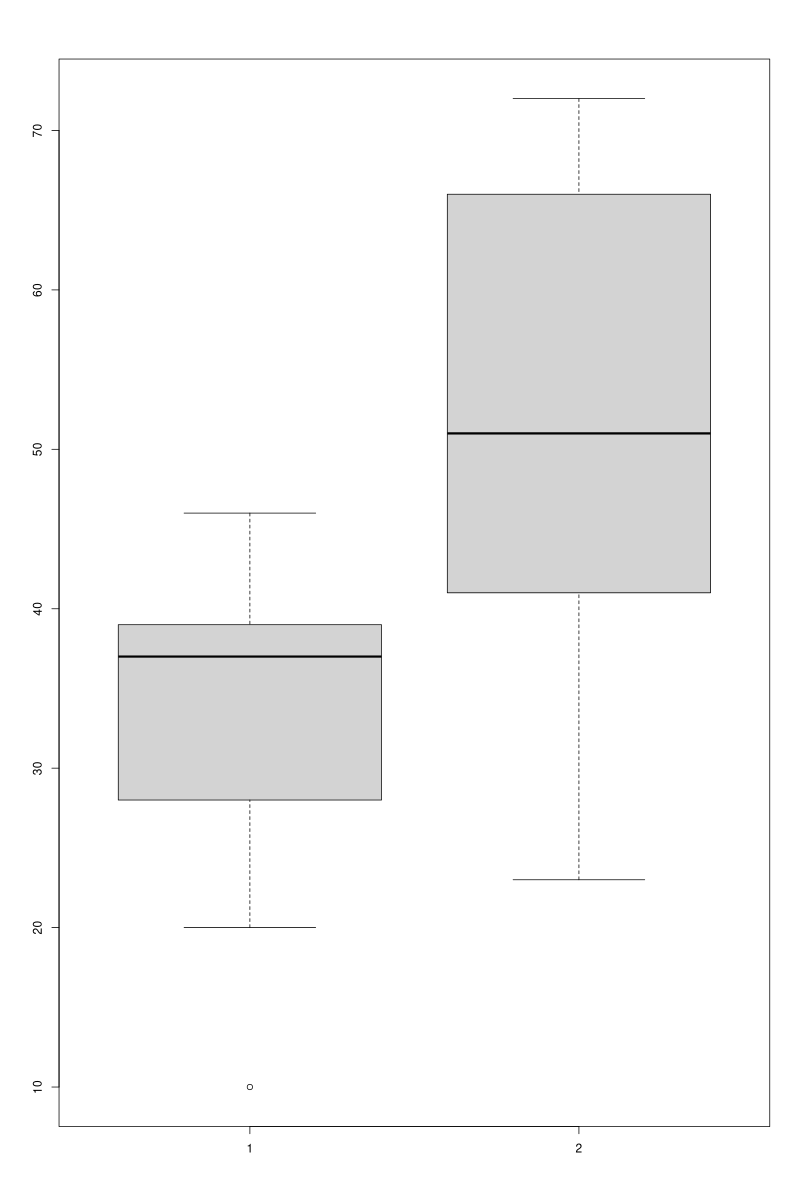
\includegraphics[scale=0.2]{img/72.png}
\end{minipage}
\begin{minipage}{0.58\textwidth}
	Observing the left box plot representing the PTSD category, it is most interesting that the median heavily leans to the upper whisker, indicating a negative skew. The minimum value is also an outlier, as visible on the box plot. The width of the box compared to the whisker indicates a fair variability ($s_{\text{PTSD}} \approx 9.93$) in the dataset.

	Now observe the right box plot representing the healthy category. Because the median leans towards the bottom, we can see the distribution is slightly positively skewed. No outliers are visible. The width of the box is relatively large, indicating a high variability ($s_{\text{Healthy}} \approx 14.86$).
\end{minipage}
\newpage
\begin{problem}{73}
	The article \textbf{``Can We Really Walk Straight?'' (\textit{Amer. J. of Physical Anthropology}, 1992: 19-27)} reported on an experiment in which each of 20 healthy men was asked to walk as straight as possible to a target 60 m away at normal speed. Consider the folloing observations on cadence (number of strides per second)
	\begin{center}
		\begin{tabular}{cccccccccc}
			.95 & .85 & .92 & .95 & .93 & .86 & 1.00 & .92 & .85 & .81 \\
			.78 & .93 & .93 & 1.05 & .93 & 1.06 & 1.06 & .96 & .81 & .96
		\end{tabular}
	\end{center}
	Use the methods developed in this chapter to summarize the data; include an interpretation or discussion wherever appropriate.
\end{problem}

Using box plots, we obtain the following:

\begin{minipage}{0.4\textwidth}
	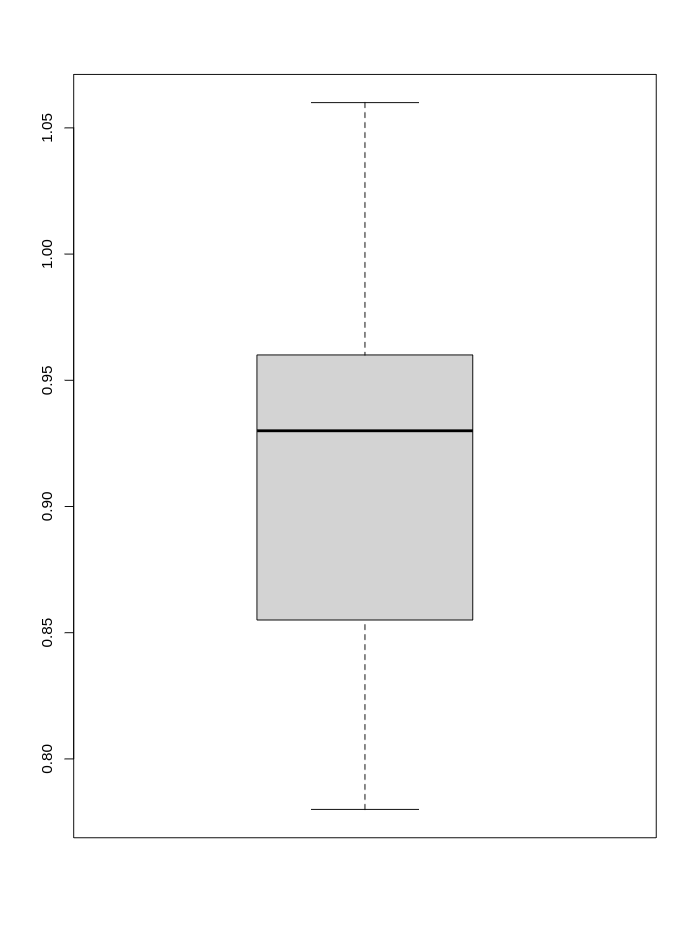
\includegraphics[scale=0.25]{img/73.png}
\end{minipage}
\begin{minipage}{0.52\textwidth}
	We can observe that the median tends towards the upper end, which may suggest a negatively skewed distribution and thus indicates a fair number of people have a cadence on the higher end. The width of the box relative to the whisker length suggests a good variability of the dataset (more specifically, $s \approx 0.08$). By the 68--95--99.7 rule, one may interpret that approximately 68\% of healthy men have a cadence of $\overline{x} \pm s \approx 0.93 \pm 0.08$. The dataset contains no outlier.
\end{minipage}

\begin{problem}{74}
	The \textbf{mode} of a numerical data set is the value that occurs most frequently in the set.
	\begin{tasks}[label=\textbf{\alph*.}]
		\task Determine the mode for the cadence data given in Exercise 73.
		\task For a categorical sample, how would you define the modal category?
	\end{tasks}
\end{problem}

\paragraph{\textbf{a.}} Ordering the data set in an increasing order, we obtain
\begin{center}
	\begin{tabular}{cccccccccc}
		.78 & .81 & .81 & .85 & .85 & .86 & .92 & .92 & .93 & .93 \\
		.93 & .93 & .95 & .95 & .96 & .96 & .00 & 1.05 & 1.06 & 1.06
	\end{tabular}
\end{center}
One can see that the mode is thus .93.

\paragraph{\textbf{b.}} For a categorical sample, the modal category is the categorical value that occurs most frequently in the data set.

\begin{problem}{75}
	Specimens of three different types of rope wire were selected, and the fatigue limit (MPa) was determined for each specimen, resulting in the accompanying data.
	\begin{description}[style=multiline, leftmargin=1.5cm, font=\normalfont\textit]
		\item[Type 1] 350 \quad 350 \quad 350 \quad 358 \quad 370 \quad 370 \quad 370 \quad 371 \quad 371 \quad 372 \quad 372 \quad 384 \quad 391 \quad 391 \quad 392
		\item[Type 2] 350 \quad 354 \quad 359 \quad 363 \quad 365 \quad 368 \quad 369 \quad 371 \quad 373 \quad 374 \quad 376 \quad 380 \quad 383 \quad 388 \quad 392
		\item[Type 3] 350 \quad 361 \quad 362 \quad 364 \quad 364 \quad 365 \quad 366 \quad 371 \quad 377 \quad 377 \quad 377 \quad 379 \quad 380 \quad 380 \quad 392
	\end{description}
	\begin{tasks}[label=\textbf{\alph*.}]
		\task Construct a comparative boxplot, and comment on similarities and differences.
		\task Construct a comparative dotplot (a dotplot for each sample with a common scale). Comment on similarities and differences.
		\task Does the comparative boxplot of part (a) give an informative assessment of similarities and differences? Explain your reasoning.
	\end{tasks}
\end{problem}

\paragraph{\textbf{a.}} The comparative boxplot of the three specimen types is illustrated as follows.

\begin{minipage}{0.38\textwidth}
	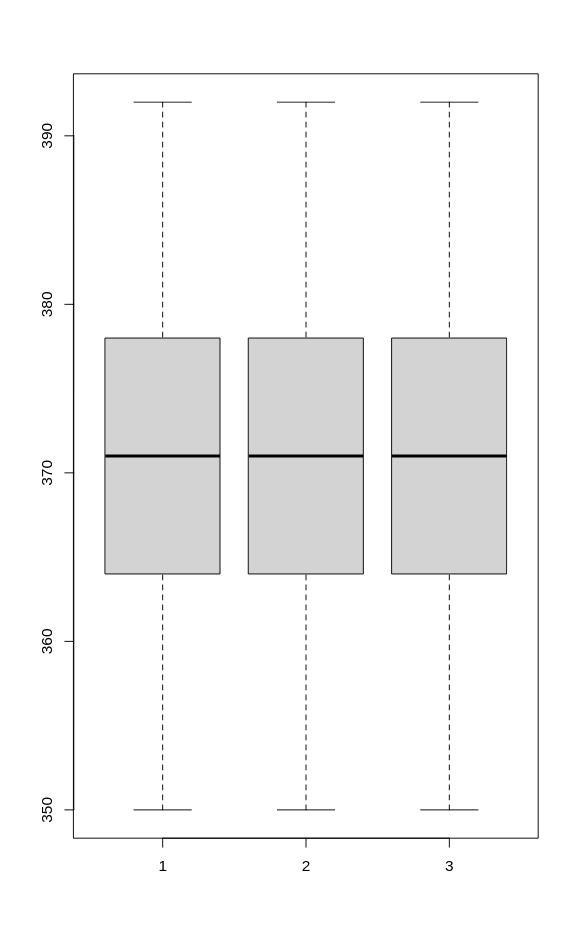
\includegraphics[scale=0.3]{img/75a.png}	
\end{minipage}
\begin{minipage}{0.52\textwidth}
	There is hardly any perceivable difference between three datasets. The boxplot of three datasets share the same total range and interquartile range, as well as sharing a roughly symmetrical distribution, and the box widths show a fair variability in all distributions. There are no outliers visible.
\end{minipage}

\paragraph{\textbf{b.}} The comparative dotplot of the three specimen types is illustrated as follows.

\begin{minipage}{0.38\textwidth}
	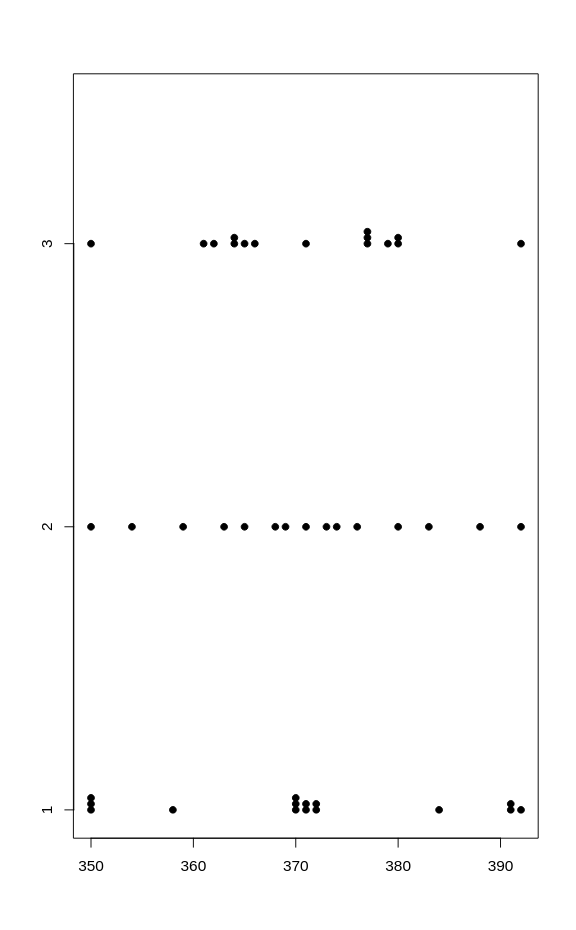
\includegraphics[scale=0.3]{img/75b.png}	
\end{minipage}
\begin{minipage}{0.52\textwidth}
	The dot plot demonstrates a similarity in the ranges of all three datasets. More specifically, the minimum and maximum values of three datasets are equal (350 and 392 respectively). In addition, all specimen types datasets share a median of 371. All three datasets display a resemblance of symmetry; one can readily verify that for each distribution, the mean is either equal or very close to the median.

	Each dataset possesses its own variability. In particular, the first dataset has a fair amount of elements at the far ends of its range ($s \approx 14.41$), the second seems more spread out but less data living at the range's ends ($s \approx 11.89$), and the third features a good aggregation of elements near its mean ($s \approx 10.54$).
\end{minipage}

\paragraph{\textbf{c.}} The comparative boxplot shown in part (a) does not give an informative assessment of similarities and differences. This is due to the high dependence of quartiles that box plot requires; as such, for datasets whose quartile values are similar, using box plot for comparative purpose is suboptimal. This is especially true for this problem's data, where all three datasets share the exact same quartile values ($Q_1 = 364, Q_2 = 371, Q_3 = 378, Q_4 = 392$).

\begin{problem}{76}
	The three measures of center introduced in this chapter are the mean, median, and trimmed mean. Two additional measures of center that are occasionally used are the \textit{midrange}, which is the average of the smallest and largest observations, and the \textit{midfourth}, which is the average of the two fourths. Which of these five measures of center are resistant to the effects of outliers and which are not? Explain your reasoning.
\end{problem}

\paragraph{Mean.} The mean is not resistant to outliers, since its value is dependent on the actual measurement of the elements, and thus outliers may impact the final value of mean in calculation.

\paragraph{Median.} The median is the most resistant to outliers. Unlike the mean, the median is not dependent on the elements' values, but rather each of the value's relationship with others (i.e. its position when ordered).

\paragraph{Trimmed mean.} The trimmed mean is more resistant to outliers than the regular mean. Because the trimmed mean discards values at the extreme ends of the data set, it effectively ignores outliers that affect the calculation.

\paragraph{Midrange.} The midrange is the least resistant to outliers. Not only does it use the lowest and highest value in the dataset, it ignores all other elements, which renders it vulnerable to an inaccurate reflection of the distribution's measure of center.

\paragraph{Midfourth.} The midfourth is more resistant to outliers than the midrange, but it still holds the same weaknesses the midrange displays.

\begin{problem}{77}
	The authors of the article \textbf{``Predictive Model for Pitting Corrosion in Buried Oil and Gas Pipelines'' (\textit{Corrosion}, 2009: 332--342)} provided the data on which their investigation was based.
	\begin{tasks}[label=\textbf{\alph*.}]
		\task Consider the following sample of 61 observations on maximum pitting depth (mm) of pipeline specimens buried in clay loan soil.
		\begin{center}
			\begin{tabular}{ccccccccc}
				0.41 & 0.41 & 0.41 & 0.41 & 0.43 & 0.43 & 0.43 & 0.48 & 0.48 \\
				0.58 & 0.79 & 0.79 & 0.81 & 0.81 & 0.81 & 0.91 & 0.94 & 0.94 \\
				1.02 & 1.04 & 1.04 & 1.17 & 1.17 & 1.17 & 1.17 & 1.17 & 1.17 \\
				1.17 & 1.19 & 1.19 & 1.27 & 1.40 & 1.40 & 1.59 & 1.59 & 1.60 \\
				1.68 & 1.91 & 1.96 & 1.96 & 1.96 & 2.10 & 2.21 & 2.31 & 2.46 \\
				2.49 & 2.57 & 2.74 & 3.10 & 3.18 & 3.30 & 3.58 & 3.58 & 4.15 \\
				4.75 & 5.33 & 7.65 & 7.70 & 8.13 & 10.41 & 13.44
			\end{tabular}
		\end{center}
		Construct a stem-and-leaf display in which the two largest values are shown in a last row labeled HI.
		\task Refer back to (a), and create a histogram based on eight classes with 0 as the lower limit of the first class and class widths of .5, .5, .5, .5, 1, 2, 5, and 5, respectively.
		\task The accompanying comparative boxplot from Minitab shows plots of pitting depth for four different types of soils. Describe its important features.
	\end{tasks}
\end{problem}

\paragraph{a.} The stem-and-leaf display of the dataset is as follows.
\begin{center}
	\begin{tabular}{c|lllllllllllllll}
		0L & 41 & 41 & 41 & 41 & 43 & 43 & 43 & 48 & 48 \\
		0H & 58 & 79 & 79 & 81 & 81 & 81 & 91 & 94 & 94 \\
		1L & 02 & 04 & 04 & 17 & 17 & 17 & 17 & 17 & 17 & 17 & 19 & 19 & 27 & 40 & 40 \\
		1H & 59 & 59 & 60 & 68 & 91 & 96 & 96 & 96 \\
		2L & 10 & 21 & 31 & 46 & 49 \\
		2H & 57 & 74 \\
		3L & 10 & 18 & 30 \\
		3H & 58 & 58 \\
		4L & 15 \\
		4H & 75 \\
		5L & 33 \\
		7H & 65 & 70 \\
		8L & 13 \\
		HI & 10.41 & 13.44
	\end{tabular}
\end{center}
Here, the stem represents the integer part, whereas the leaf represents the decimal part.
\newpage
\paragraph{b.} The histogram is given as follows.

\begin{minipage}{\linewidth}
	\begin{center}
		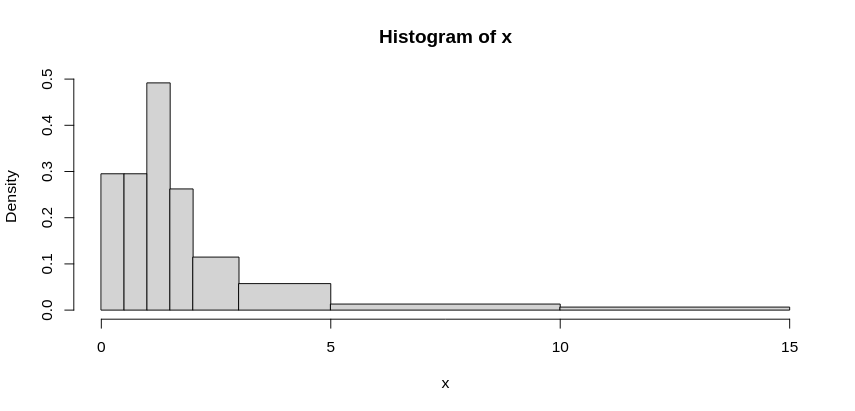
\includegraphics[width=\linewidth]{img/77b.png}
	\end{center}
\end{minipage}

\paragraph{c.} The first three box plots for the soils of type C, CL, SCL have medians tending towards the lower whiskers, suggesting positively skewed distributions. In addition, they also contain a fair number of outliers, whereas the fourth boxplot for SYCL soil does not contain any outlier. The widths of the boxes in the first two box plots are fairly large, indicating fair variabilities. In contrast, the boxes' widths in the last two box plots are relatively smaller, suggesting less variabilities. Furthermore, the long lengths of the whiskers for the first two soils suggest a good number of elements living in the ranges' ends.

\begin{problem}{78}
	Consider a sample $x_1, x_2, \dots x_n$ and suppose that the values of $\overline x$, $s^2$, and $s$ have been calculated.
	\begin{tasks}[label=\textbf{\alph*.}]
		\task Let $y_i = x_i - \overline x$ for $i = 1, \dots, n$. How do the values of $s^2$ and $s$ for the $y_i$'s compare to the corresponding values for the $x_i$'s? Explain.
		\task Let $z_i = (x_i - \overline x)/s$ for $i = 1, \dots, n$. What are the values of the sample variance and sample standard deviation for the $z_i$'s?
	\end{tasks}
\end{problem}

\paragraph{a.} Denote by $s_x$, $s_y$ the standard deviations of $\{x_i\}$ and $\{y_i\}$ respectively. We first calculate the mean of the latter:
\[
	\overline y = \frac{\displaystyle\sum_{i = 1}^n y_i}n = \frac{\displaystyle\sum_{i = 1}^n (x_i - \overline x)}n = \frac{n\overline x - n\overline x}n = 0.
\]
Thus one can observe that
\[
	s_x = \sqrt{\frac{\displaystyle \sum_{i = 1}^n (x_i - \overline x)^2}{n - 1}} = \sqrt{\frac{\displaystyle \sum_{i = 1}^n y_i^2}{n - 1}} = s_y.
\]
We conclude that $s_y = s_x$.

\paragraph{b} Denote by $s_z$ the standard deviation of $\{z_i\}$. We first calculate its mean:
\[
	\overline z = \frac{\displaystyle\sum_{i = 1}^n z_i}n = \frac{\displaystyle\sum_{i = 1}^n \frac{(x_i - \overline x)}{s_x}}n = \frac{n\overline x - n\overline x}{s_xn} = 0.
\]
Thus one can observe that
\[
	s_x = \sqrt{\frac{\displaystyle \sum_{i = 1}^n (x_i - \overline x)^2}{n - 1}} = \sqrt{\frac{\displaystyle s_x^2\sum_{i = 1}^n z_i^2}{(n - 1)}} = s_xs_z.
\]
Therefore $s_z = 1$. Naturally, $s_z^2 = 1$.

\end{document}